
\documentclass[border=3pt,tikz]{standalone}
\tikzset{>=latex} % for LaTeX arrow head
\usetikzlibrary{fpu} % for higher floating-point precision
\pgfkeys{
  /pgf/fpu/output format=fixed, % fpu floating-point format
  /pgf/number format/precision=2 % two decimals
}
\begin{document}
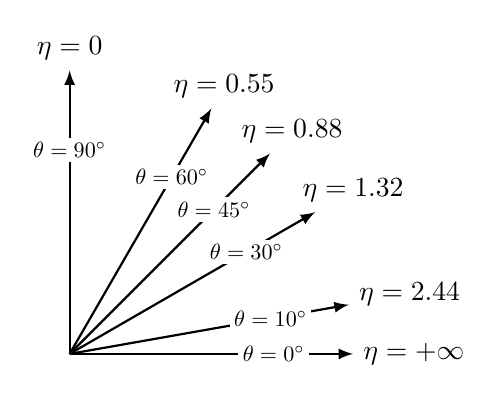
\begin{tikzpicture}[scale=3]
  \foreach \t in {90,60,45,30,10,0}{
    \ifnum \t = 0
      \def\e{+\infty} % infinity symbol
    \else
      \pgfkeys{/pgf/fpu=true} % increase floating-point precision in computation
      \pgfmathparse{-ln(tan(\t/2))} % pseudorapidity
      \pgfkeys{/pgf/fpu=false} % turn off to avoid interference with following
      \pgfmathroundtozerofill{\pgfmathresult} % round with trailing zeroes
      \pgfmathsetmacro\e{\t==90?0:\pgfmathresult} % no trailing zeroes for theta = 0
    \fi
    \draw[->,thick] % eta lines
      (0,0) -- (\t:1.2) node[anchor=180+\t,black] {$\eta=\e$}
      node[black,pos=0.72,fill=white,scale=0.8,inner sep=2] {$\theta=\t^\circ$};
  }
\end{tikzpicture}
\end{document}
